\documentclass{article}
\usepackage{v-test-paper}
\newenvironment{solution}{\par\noindent\color{red!85!black}$\Rightarrow$\vspace{0em}}{}
\title{\textsc{JEE Advanced 2012 Paper-II\\Physics}}
\date{}

\usepackage{mathtools}
\begin{document}
\maketitle
\begin{enumerate}
    
\begin{enumerate}
    \item In a historical experiment to determine Planck's constant, a metal surface was irradiated with light of different wavelengths. The emitted photoelectron energies were measured by applying a stopping potential. The relevant data for the wavelength (\(\lambda\)) of incident light and the corresponding stopping potential (\(V_0\)) are given below:
    \begin{center}
        \begin{tabular}{ccc}
        \hline
        \(\lambda (\mu m)\) & \(V_0 (Volt)\) \\
        \hline
        0.3 & 2.0 \\
        0.4 & 1.0 \\
        0.5 & 0.4 \\
        \hline
        \end{tabular}
    \end{center}
    Given that \( c = 3 \times 10^8 m\ s^{-1} \) and \( e = 1.6 \times 10^{-19} C \), Planck's constant (in units of J s) found from such an experiment is
    \begin{tasks}(2)
        \task \( 6.0 \times 10^{-34} \)
        \task \( 6.4 \times 10^{-34} \)
        \task \( 6.6 \times 10^{-34} \)
        \task \( 6.8 \times 10^{-34} \)
    \end{tasks}
\end{enumerate}

    
\item In the arrangement of Fig. 1.9 the masses \( m_0 \), \( m_1 \), and \( m_2 \) of bodies are equal, the masses of the pulley and the threads are negligible, and there is no friction in the pulley. Find the acceleration \( w \) with which the body \( m_0 \) comes down, and the tension of the thread binding together the bodies \( m_1 \) and \( m_2 \), if the coefficient of friction between these bodies and the horizontal surface is equal to \( k \). Consider possible cases.
    \begin{center}
        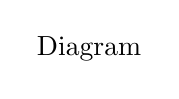
\begin{tikzpicture}
            \node at (0, 0) {Diagram};
        \end{tikzpicture}
    \end{center}

    
\begin{enumerate}
    \item A current carrying wire heats a metal rod. The wire provides a constant power (P) to the rod. The metal rod is enclosed in an insulated container. It is observed that the temperature (T) in the metal rod changes with time (t) as
    \[
    T(t) = T_0(1 + \beta t)^{\frac{1}{4}},
    \]
    where \(\beta\) is a constant with appropriate dimension while \(T_0\) is a constant with dimension of temperature. The heat capacity of the metal is;
        \begin{tasks}(2)
            \task \(\frac{4P(T(t)-T_0)^3}{\beta^4 T_0}\)
            \task \(\frac{4P(T(t)-T_0)^4}{\beta^4 T_0^5}\)
            \task \(\frac{4P(T(t)-T_0)^2}{\beta^4 T_0^3}\)
            \task \(\frac{4P(T(t)-T_0)}{\beta^4 T_0^2}\)
        \end{tasks}
\end{enumerate}

    
\item A point moves rectilinearly in one direction. Fig. 1.1 shows the distance \( s \) traversed by the point as a function of the time \( t \).
    \begin{center}
        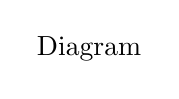
\begin{tikzpicture}
            \node at (0, 0) {Diagram}; % Replace this with the actual TikZ code for the diagram.
        \end{tikzpicture}
    \end{center}
Using the plot find:
\begin{itemize}
    \item the average velocity of the point during the time of motion;
    \item the maximum velocity;
    \item the time moment \( t_0 \) at which the instantaneous velocity is equal to the mean velocity averaged over the first \( t_0 \) seconds.
\end{itemize}

    \item A disc of mass \( m = 50 \) g slides with the zero initial velocity down an inclined plane set at an angle \( \alpha = 30^\circ \) to the horizontal; having traversed the distance \( l = 50 \) cm along the horizontal plane, the disc stops. Find the work performed by the friction forces over the whole distance, assuming the friction coefficient \( k = 0.15 \) for both inclined and horizontal planes.
    \begin{center}
        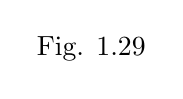
\begin{tikzpicture}
            \node at (0, 0) {Fig. 1.29};
        \end{tikzpicture}
    \end{center}\begin{solution}
    \begin{center}
        \begin{tikzpicture}
            \pic at (0, 0) {frame=3cm};
        \end{tikzpicture}
    \end{center}

    \begin{align*}
        \intertext{Let \(s\) be the distance covered by the disk along the incline, from the equation of increment of mechanical energy of the disk in the field of gravity: \(\Delta T + \Delta U - A_{fr}\)}
        0 + (-mgs\sin\alpha) &= -kmg\cos\alpha \cdot s - kmgl\\
        \intertext{or}
        s &= \dfrac{kl}{\sin\alpha - k\cos\alpha} \tag{1}
        \intertext{Hence the sought work}
        A_{fr} &= -kmg[s \cos\alpha + l]\\
        A_{fr} &= -\dfrac{klmg}{1 - k \cos\alpha} \quad \text{(using Eq. 1)}
        \intertext{On putting the values}
        A_{fr} &= -0.05 \, \text{J}
    \end{align*}
\end{solution}
    \item Two bars of masses $m_1$ and $m_2$ connected by a non-deformed light spring rest on a horizontal plane. The coefficient of friction between the bars and the surface is equal to $k$. What minimum constant force has to be applied in the horizontal direction to the bar of mass $m_1$ in order to shift the other bar?
\begin{solution}
    \begin{center}
        \begin{tikzpicture}
            \pic at (0, 0) {frame=3cm};
        \end{tikzpicture}
    \end{center}

    \begin{align*}
        \intertext{Let \(x\) be the compression in the spring when the bar \(m_2\) is about to shift. Therefore at this moment spring force on \(m_2\) is equal to the limiting friction between the bar \(m_2\) and horizontal floor. Hence}
        \kappa x &= km_2 g \quad \text{[where \(\kappa\) is the spring constant (say)]} \quad \tag{1}
        \intertext{For the block \(m_1\) from work-energy theorem:}
        A &= \Delta T = 0 \text{ for minimum force. (A here includes the work done in stretching the spring.)}
        \intertext{So,}
        Fx - \dfrac{1}{2} \kappa x^2 - km_1 g x &= 0 \quad \text{or} \quad \kappa \dfrac{x}{2} = F - km_1 g \quad \tag{2}
        \intertext{From Eqs. (1) and (2),}
        F &= kg \left(m_1 + \dfrac{m_2}{2}\right)
    \end{align*}
\end{solution}

    
\begin{enumerate}
    \item Two loudspeakers \(M\) and \(N\) are located 20 m apart and emit sound at frequencies 118 Hz and 121 Hz, respectively. A car is initially at a point \(P\), 1800 m away from the midpoint \(Q\) of the line \(MN\) and moves towards \(Q\) constantly at 60 km/hr along the perpendicular bisector of \(MN\). It crosses \(Q\) and eventually reaches a point \(R\), 1800 m away from \(Q\). Let \(v_P\), \(v_Q\) and \(v_R\) be the beat frequencies measured by a person sitting in the car at time \(t\). Let \(v(t)\) represent the beat frequency measured by a person sitting in the car at time \(t\). The speed of sound in air is 330 m s\(^{-1}\). Which of the following statement(s) is(are) true regarding the sound heard by the person?
        \begin{tasks}(1)
            \task \(v_P + v_R = 2 v_Q\)
            \task The rate of change in beat frequency is maximum when the car passes through \(Q\)
            \task The plot below represents schematically the variation of beat frequency with time (with a labeled diagram indicating points \(P\), \(Q\), and \(R\).)
            \task The plot below represents schematically the variation of beat frequency with time (with a labeled diagram indicating points \(P\), \(Q\), and \(R\).)
        \end{tasks}
\end{enumerate}
\begin{center}
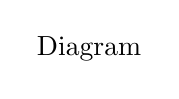
\begin{tikzpicture}
\node {Diagram};
\end{tikzpicture}
\end{center}

    
\item A spherical metal shell A of radius $R_A$ and a solid metal sphere B of radius $R_B$ ($R_B < R_A$) are kept far apart and each is given charge $`+Q'$. Now they are connected by a thin metal wire. Then
    \begin{tasks}(2)
        \task $E_{\text{inside}}^A = 0$
        \task $Q_A > Q_B$
        \task $\frac{\sigma_A}{\sigma_B} = \frac{R_B}{R_A}$
        \task $E_{\text{on surface}}^A < E_{\text{on surface}}^B$
    \end{tasks}

    \begin{center}
    \textsc{Paragraph for Questions 9 and 10}
\end{center}

A point charge $Q$ is moving in a circular orbit of radius $R$ in the x-y plane with an angular velocity $\omega$. This can be considered as equivalent to a loop carrying a steady current $\frac{Q\omega}{2\pi}$. 

A uniform magnetic field along the positive z-axis is now switched on, which increases at a constant rate from $0$ to $B$ in one second. Assume that the radius of the orbit remains constant. The application of the magnetic field induces an emf in the orbit. The induced emf is defined as the work done by an induced electric field in moving a unit positive charge around a closed loop. It is known that, for an orbiting charge, the magnetic dipole moment is proportional to the angular momentum with a proportionality constant $\gamma$. 

\item The magnitude of the induced electric field in the orbit at any instant of time during the time interval of the magnetic field change is
    \begin{tasks}(4)
        \task $\dfrac{BR}{4}$
        \task $\dfrac{BR}{2}$\ans
        \task $\dfrac{BR}{\pi}$
        \task $2BR$
    \end{tasks}

\item The change in the magnetic dipole moment associated with the orbit, at the end of the time interval of the magnetic field change, is
    \begin{tasks}(4)
        \task $-\gamma BQR^2$
        \task $-\dfrac{\gamma BQR^2}{2}$\ans
        \task $\dfrac{BQR^2}{\gamma}$
        \task $\gamma BQR^2$
    \end{tasks}
    \begin{center}
    \textsc{Paragraph for Questions 11 and 12}
\end{center}

The $\beta$-decay process, discovered around 1900, is basically the decay of a neutron $(n)$. In the laboratory, a proton $(p)$ and an electron $(e^-)$ are observed as the decay products of the neutron. Therefore, considering the decay of a neutron as a two-body decay process, it was predicted theoretically that the kinetic energy of the electron should be a constant. But experimentally, it was observed that the electron kinetic energy has a continuous spectrum. Considering a three-body decay process, i.e. $n \rightarrow p + e^- + \bar{\nu}_e$, around 1930, Pauli explained the observed electron energy spectrum. Assuming the anti-neutrino $(\bar{\nu}_e)$ to be massless and possessing negligible energy, and the neutron to be at rest, momentum and energy conservation principles are applied. From this calculation, the maximum kinetic energy of the electron is $0.8 \times 10^6$ eV. The kinetic energy carried by the proton is only the recoil energy.

\item What is the maximum energy of the anti-neutrino?
    \begin{tasks}(2)
        \task Zero.
        \task Much less than $0.8 \times 10^6$ eV.
        \task Nearly $0.8 \times 10^6$ eV.
        \task Much larger than $0.8 \times 10^6$ eV.
    \end{tasks}

\item If the anti-neutrino had a mass of $3 eV/c^2$ (where $c$ is the speed of light) instead of zero mass, what should be the range of the kinetic energy, $K$, of the electron?
    \begin{tasks}(2)
        \task $0 \leq K \leq 0.8 \times 10^6$ eV
        \task $3.0 eV \leq K \leq 0.8 \times 10^6$ eV
        \task $3.0 eV \leq K < 0.8 \times 10^6$ eV
        \task $0 \leq K < 0.8 \times 10^6$ eV
    \end{tasks}
    \begin{center}
    \textsc{Paragraph for Questions 13 and 14}
\end{center}

A small block of mass 1 kg is released from rest at the top of a rough track. The track is a circular arc of radius 40 m. The block slides along the track without toppling and a frictional force acts on it in the direction opposite to the instantaneous velocity. The work done in overcoming the friction up to the point \( Q \), as shown in the figure below, is 150 J. (Take the acceleration due to gravity, \( g = 10\ m/s^2 \)).

\begin{center}
    \begin{tikzpicture}
        % Track
        \draw[thick] (0,0) arc (180:240:2cm);
        % Block sliding marks
        \draw[dashed] (0,0) -- (1.73, -1); % Extended line that fades
        % Radius lines
        \draw[dashed] (0,0) -- (-2,0) node[midway, above] {\( R \)};
        \draw[dashed] (1.73, -1) -- (0,0) node[midway, above right] {\( R \)};
        % Angle
        \draw (0,-0.5) arc (270:300:0.5cm) node[midway, right] {\( 30^\circ \)};
        % Point labels
        \filldraw[black] (0,0) circle (2pt) node[above left] {\( P \)};
        \filldraw[black] (1.73, -1) circle (2pt) node[below right] {\( Q \)};
        % Axis labels
        \draw[->] (-2.5,0) -- (2.5,0) node[right] {\( x \)};
        \draw[->] (0,0) -- (0,2.5) node[above] {\( y \)};
    \end{tikzpicture}
\end{center}

\item The speed of the block when it reaches the point \( Q \) is
    \begin{tasks}(4)
        \task \( 5\ m/s^{-1} \)
        \task \( 10\ m/s^{-1} \)
        \task \( 10\sqrt{3}\ m/s^{-1} \)
        \task \( 20\ m/s^{-1} \)
    \end{tasks}
    
\item The magnitude of the normal reaction that acts on the block at the point \( Q \) is
    \begin{tasks}(4)
        \task \( 7.5\ N \)
        \task \( 8.6\ N \)
        \task \( 11.5\ N \)
        \task \( 22.5\ N \)
    \end{tasks}
    
\begin{enumerate}
    \item A train S1, moving with a uniform velocity of 108 km/h, approaches another train S2 standing on a platform. An observer O moves with a uniform velocity of 36 km/h towards S2, as shown in figure. Both the trains are blowing whistles of same frequency 120 Hz. When O is 600 m away from S2 and distance between S1 and S2 is 800 m, the number of beats heard by O is \_\_\_\_\_\_\_\_\_. \\
    [Speed of the sound = 330 m/s]
    \begin{center}
        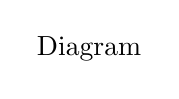
\begin{tikzpicture}
            \node {Diagram};
        \end{tikzpicture}
    \end{center}
\end{enumerate}

    \item From the photoelectric effect experiment, following observations are made. Identify which of these are correct.
    \begin{tasks}(1)
        \task The stopping potential depends only on the work function of the metal.
        \task The saturation current increases as the intensity of incident light increases.
        \task The maximum kinetic energy of a photo electron depends on the intensity of the incident light.
        \task Photoelectric effect can be explained using wave theory of light.
    \end{tasks}
    
Choose the correct answer from the options given below:
\begin{tasks}(2)
        \task B, C only
        \task A, C, D only
        \task A, B, D only
        \task B only
    \end{tasks}
     1. A stationary tuning fork is in resonance with an air column in a pipe. If the tuning fork is moved with a speed of \(2\text{ m s}^{-1}\) in front of the open end of the pipe and parallel to it, the length of the pipe should be changed for the resonance to occur with the moving tuning fork. If the speed of sound in air is \(320\text{ m s}^{-1}\), the smallest value of the percentage change required in the length of the pipe is _____.

\begin{center}
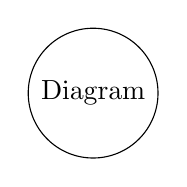
\begin{tikzpicture}
  \node [draw, shape=circle] {Diagram};
\end{tikzpicture}
\end{center}
     \item A circular disk of radius \(R\) carries surface charge density \(\sigma(r) = \sigma_0 \left(1 - \frac{r}{R}\right)\), where \(\sigma_0\) is a constant and \(r\) is the distance from the center of the disk. Electric flux through a large spherical surface that encloses the charged disk completely is \(\Phi_0\). Electric flux through another spherical surface of radius \(R-\frac{r}{4}\) and concentric with the disk is \(\Phi\). Then the ratio \(\frac{\Phi}{\Phi_0}\) is \underline{\hspace{2.5 cm}}.

 \begin{solution}
    \begin{align*}
        \intertext{Total charge on the disk, \(Q\), is obtained by integrating the surface charge density over the area of the disk,}
        Q &= \int_0^{2\pi} \int_0^R \sigma(r) r \, dr \, d\theta \\
        &= \int_0^{2\pi} \int_0^R \sigma_0 \left(1 - \frac{r}{R}\right) r \, dr \, d\theta \\
        &= \sigma_0 \int_0^{2\pi} \left(\int_0^R r - \frac{r^2}{R} \, dr\right) d\theta \\
        &= \sigma_0 \int_0^{2\pi} \left(\frac{R^2}{2} - \frac{R^3}{3R}\right) d\theta \\
        &= \sigma_0 (2\pi) \left(\frac{R^2}{2} - \frac{R^2}{3}\right) \\
        &= \sigma_0 (2\pi) \frac{R^2}{6} \\
        &= \frac{\sigma_0 \pi R^2}{3}
        \intertext{The electric flux \(\Phi_0\) through a large spherical surface enclosing the disk is given by,}
        \Phi_0 &= \frac{Q}{\varepsilon_0} \\
        &= \frac{\sigma_0 \pi R^2}{3\varepsilon_0}
        \intertext{The electric flux \(\Phi\) through a spherical surface of radius \(R-\frac{r}{4}\) is given by,}
        \Phi &= \frac{Q'}{\varepsilon_0}
        \intertext{where \(Q'\) is the charge inside the sphere of radius \(R-\frac{r}{4}\). Since the sphere is concentric with the disk, we need to find charge within radius \(R-\frac{r}{4}\),}
        Q' &= \int_0^{2\pi} \int_0^{R-\frac{r}{4}} \sigma(r) r \, dr \, d\theta \\
        &= \sigma_0 \int_0^{2\pi} \left(\int_0^{R-\frac{r}{4}} r - \frac{r^2}{R} \, dr\right) d\theta \\
        &= \sigma_0 \int_0^{2\pi} \left(\frac{(R-\frac{r}{4})^2}{2} - \frac{(R-\frac{r}{4})^3}{3R}\right) d\theta \\
        &= \sigma_0 (2\pi) \frac{(R-\frac{r}{4})^2}{6} \\
        &= \frac{\sigma_0 \pi (R-\frac{r}{4})^2}{3}
        \intertext{So, the ratio \(\frac{\Phi}{\Phi_0}\) is,}
        \frac{\Phi}{\Phi_0} &= \frac{\frac{\sigma_0 \pi (R-\frac{r}{4})^2}{3\varepsilon_0}}{\frac{\sigma_0 \pi R^2}{3\varepsilon_0}} \\
        &= \frac{(R-\frac{r}{4})^2}{R^2} \\
        &= \frac{R^2 - \frac{rR}{2} + \frac{r^2}{16}}{R^2} \\
        &= 1 - \frac{r}{2R} + \frac{r^2}{16R^2}
        \intertext{This is the required ratio of the electric fluxes.}
    \end{align*}
\end{solution}
    
    \item A horizontal circular platform of radius 0.5 m and mass 0.45 kg is free to rotate about its axis. Two massless spring toy-guns, each carrying a steel ball of mass 0.05 kg are attached to the platform at a distance 0.25 m from the centre on its either sides along its diameter (see figure). Each gun simultaneously fires the balls horizontally and perpendicular to the diameter in opposite directions. After leaving the platform, the balls have horizontal speed of 9 m\textsuperscript{-1} with respect to the ground. The rotational speed of the platform in\textsuperscript{-1} after the balls leave the platform is \underline{\hspace{2.5 cm}}.

    \begin{center}
        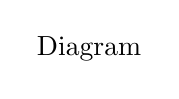
\begin{tikzpicture}
            \node {Diagram};
        \end{tikzpicture}
    \end{center}

    \item A particle of unit mass is moving along the x-axis under the influence of a force and its total energy is conserved. Four possible forms of the potential energy of the particle are given in Column I($a$ and $U_0$ are constants). Match the potential energy functions in Column I with the corresponding statement(s) in Column II.
\begin{center}
    \renewcommand{\arraystretch}{3}
    \begin{table}[h]
        \centering
        \begin{tabular}{p{0.25cm}p{5cm}|p{0.25cm}p{8cm}}
        \hline
        & Column I & & Column II \\
        \hline
        (A) & \( U_1(x) = \frac{U_0}{2} \left[ 1 - \left( \frac{x}{a} \right)^2 \right]^2 \) & (P) & The force acting on the particle is zero at \( x = a \). \\
        (B) & \( U_2(x) = \frac{U_0}{2} \left( \frac{x}{a} \right)^2 \) & (Q) & The force acting on the particle is zero at \( x = 0 \). \\
        (C) & \( U_3(x) = \frac{U_0}{2} \left( \frac{x}{a} \right)^2 \exp \left[ - \left( \frac{x}{a} \right)^2 \right] \) & (R) & The force acting on the particle is zero at \( x = -a \). \\
        (D) & \( U_4(x) = \frac{U_0}{2} \left[ \frac{x}{a} - \frac{1}{3} \left( \frac{x}{a} \right)^3 \right] \) & (S) & The particle experiences an attractive force towards \( x = 0 \) in the region \( |x| < a \). \\
         &  & (T) & The particle with total energy \( \frac{U_0}{4} \) can oscillate about the point \( x = -a \). \\
        \hline
        \end{tabular}
    \end{table}
\end{center}
\begin{solution}
    \begin{align*}
        \intertext{The force acting on the particle can be found by taking the negative derivative of the potential energy function with respect to $x$.}
        \intertext{For option (A):}
        F_1(x) &= -\dfrac{dU_1}{dx} = -\dfrac{d}{dx} \left[ \dfrac{U_0}{2} \left(1-\dfrac{x^2}{a^2}\right)^2 \right]\\
        &= -U_0 \left(\dfrac{x}{a^2}\right) \left(1-\dfrac{x^2}{a^2}\right)\\
        \intertext{The force acting on the particle is zero at \(x=0\) and \(x=\pm a\) which corresponds to option (Q) and (P)(R).}
        \intertext{For option (B):}
        F_2(x) &= -\dfrac{dU_2}{dx} = -\dfrac{d}{dx} \left[ \dfrac{U_0}{2} \left(\dfrac{x}{a}\right)^2 \right]\\
        &= -U_0 \left(\dfrac{x}{a^2}\right)\\
        \intertext{The force acting on the particle is zero at \(x=0\) which corresponds to option (Q).}
        \intertext{For option (C):}
        F_3(x) &= -\dfrac{dU_3}{dx} = -\dfrac{d}{dx} \left[ \dfrac{U_0}{2} \left(\dfrac{x}{a}\right)^2 \exp\left(-\dfrac{x^2}{a^2}\right) \right]\\
        &= -U_0 \left(\dfrac{x}{a^2}\right) \exp\left(-\dfrac{x^2}{a^2}\right) \left(1 - 2\dfrac{x^2}{a^2}\right)\\
        \intertext{The force acting on the particle is zero at \(x=0\) and \(x=\pm a/\sqrt{2}\) which corresponds to option (Q).}
        \intertext{For option (D):}
        F_4(x) &= -\dfrac{dU_4}{dx} = -\dfrac{d}{dx} \left[ \dfrac{U_0}{2} \left(\dfrac{x}{a} - \dfrac{1}{3}\left(\dfrac{x}{a}\right)^3 \right) \right]\\
        &= U_0 \left(\dfrac{1}{a} - \dfrac{x^2}{a^3}\right)\\
        \intertext{The force acting on the particle is zero at \(x=\pm a\) which corresponds to option (P) and (R). Also, in the region \(|x|<a\) the term inside the parentheses is positive, so the force acting on the particle is towards \(x=0\) which corresponds to option (S).}
    \end{align*}
\end{solution}
\end{enumerate}
\end{document}